\documentclass{article}
\usepackage[utf8]{inputenc}

\usepackage{natbib}
\usepackage{graphicx}
\usepackage{amsmath}
\usepackage{listings}

\title{\underline{\textit{\Large{Assignment 8: THE DIGITAL FOURIER TRANSFORM}}}}
\author{\textit{ SHAILESH PUPALWAR, EE20B100 }}



\begin{document}

\maketitle

\section{Introduction}
This assignment deals with Digital Fourier Transform(DFT) and how it is implemented in python using Numpy's FFT module. FFT is an implementation of the DFT.  We also attempt to approximate the continuous time fourier transform of a gaussian by windowing and sampling in time domain, and then taking the DFT. And during analysis, the graphs are plotted.

\section {FFT and IFFT}
We find the Fourier transform and invert it back to the time domain for a random signal. And then find maximum error to test the reconstruction.
\newline\newline
The maximum error obtained from the below code = 2.7781647035173285e-16\newline\newline

\lstset{language=Python}
\lstset{frame=lines}
\lstset{label={lst:code_direct}}
\lstset{basicstyle=\footnotesize}
\newline
\newline
\begin{lstlisting}
x=rand(100)
X=fft(x)
y=ifft(X)
c_[x,y]
print (abs(x-y).max())
\end{lstlisting}

\section{Spectrum of $sin(5t)$}
The solution for this is already a part of the assignment. As expected the phase fro some values near the peaks is non zero. To fix this we sample the input signal at an appropriate frequency. We also shift the phase plot so that it goes from $-\pi$ to $\pi$. To do this we write a helper function

\begin{lstlisting}
x = linspace(0, 2*pi, 129); x = x[:-1]
y = sin(5*x)
Y0 = fftshift(fft(y))/128.0
w0 = linspace(-64, 63, 128)

figure(0)

# Magnitude Plot
subplot(2, 1, 1)  
plot(w0, abs(Y0), lw = 2) # Magnitude plot
xlim([-10, 10]) # x(i.e., w{omega}) - axis limit 
ylabel("|Y|", size = 16)
title("Spectrum of sin(5t)")
grid(True)

# Phase plot
subplot(2, 1, 2)
plot(w0, angle(Y0), 'ro', lw = 2) # Phase plot for all w 
ii = where(abs(Y0) > 1e-3)
plot(w0[ii], angle(Y0[ii]), 'go', lw = 2) 
xlim([-10, 10])
ylabel("Phase of Y", size = 16)
xlabel("k", size = 16)
grid(True)
show()
\end{lstlisting}

As expected we get 2 peaks at +5 and -5 with height 0.5. The phases of the peaks are at $\frac{\pi}{2}$ and $-\frac{\pi}{2}$ are also expected based on the expansion of a sine wave ie:
\begin{equation}
sin(5t) = 0.5(\frac{e^{5t}}{j}-\frac{e^{-5t}}{j})
\end{equation}
\begin{figure}[h!]
\centering
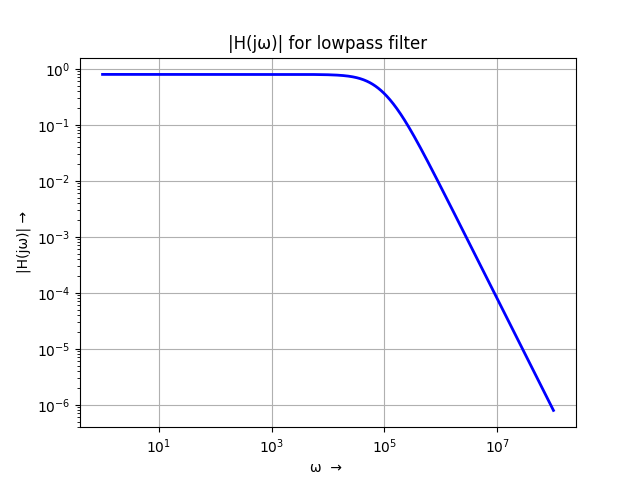
\includegraphics[scale=0.6]{Figure_0.png}
\caption{Spectrum of $f(t) =  sin(5t) }
\label{fig:universe}
\end{figure}


\section{Amplitude Modulation}
Consider the signal:\newline
\begin{equation}
f(t) = (1+0.1\cos(t))\cos(10t)    
\end{equation}

We  expect  a  shifted  set  of  spikes,  with  a  main  impulse  and  two  side impulses on each side.  This is because,
\begin{equation}
    0.1cos(10t)cos(t) = 0.05(cos11t+cos9t)= 0.025(e^{11tj}+e^{9tj}+e^{-11tj}+e^{-9tj})
\end{equation}
In  order  to  see  even  the  side  peaks,  the  frequency  resolution  has  to  beimproved.  We can do so by keeping the number of samples constant andincreasing the range in the time domain.  The following spectrum is obtained.
The python code for this part is shown below:-
\begin{lstlisting}
t1 = linspace(-4*pi, 4*pi, 513); t1 = t1[:-1] 
y1 = (1 + 0.1*cos(t1))*cos(10*t1) 
Y1 = fftshift(fft(y1))/512.0  
w1 = linspace(-64,64,513); w1 = w1[:-1]

figure(1)


# Magnitude Plot
subplot(2, 1, 1)
plot(w1, abs(Y1), lw = 2)
xlim([-15, 15])
ylabel("|Y|", size = 16)
title("Spectrum of (1 + 0.1cos(t))cos(10t)")
grid(True)

# Phase plot 
subplot(2, 1, 2)
plot(w1, angle(Y1), 'ro', lw = 2)
xlim([-15, 15])
ylabel("Phase of Y", size = 16)
xlabel("ω", size = 16)
grid(True)
show()
\end{lstlisting}
\begin{figure}[h!]
\centering
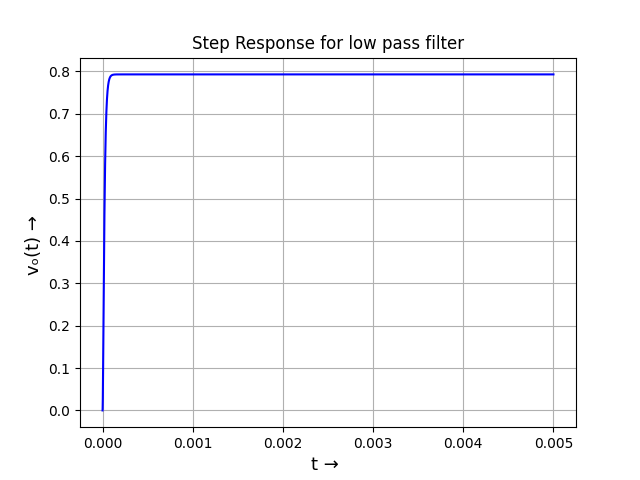
\includegraphics[scale=0.6]{Figure_1.png}
\caption{Spectrum of $f(t) = (1+0.1\cos(t))\cos(10t)$ with a higher number of samples}
\label{fig:universe}
\end{figure}
\clearpage
\section{Spectrum of $sin^3(t)$}
This signal can be expressed as a sum of sine waves using this identity:\newline
$\sin^3(t) = \frac{3}{4}\sin(t) - \frac{1}{4}\sin(3t)$\newline
We expect 2 peaks at frequencies 1 and 3, and phases similar to that expected from a sum of sinusoids.
The python code for this part:-
\begin{lstlisting}
t3 = linspace(-4*pi, 4*pi, 513); t3 = t3[:-1]
y3 = (sin(t3))**3
Y3 = fftshift(fft(y3))/512.0
w3 = linspace(-64, 64, 513); w3 = w3[:-1]
figure(3)
# Magnitude Plot
subplot(2, 1, 1)
plot(w3, abs(Y3), lw = 2)
xlim([-15, 15])
ylabel("|Y|", size = 16)
title("Spectrum of sin\u00B3(t)")
grid(True)
# Phase Plot
subplot(2, 1, 2)
plot(w3, angle(Y3), 'ro', lw = 2)
xlim([-15, 15])
ylabel("Phase of Y", size = 16)
xlabel("ω", size = 16)
grid(True)
show()
\end{lstlisting}
\begin{figure}[h!]
\centering
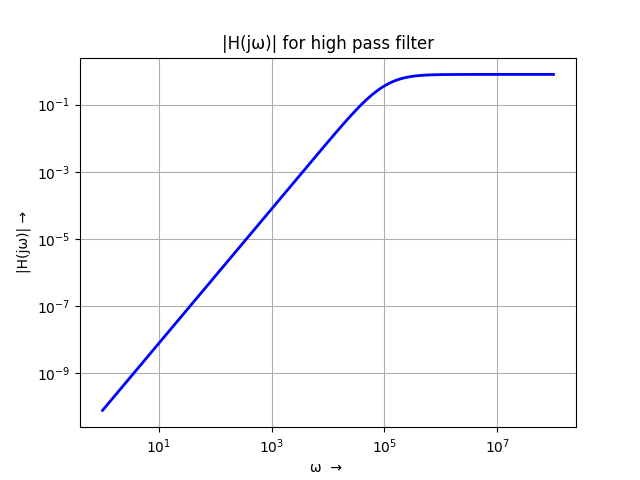
\includegraphics[scale=0.6]{Figure_3.png}
\caption{Spectrum of $f(t) = sin^3(t)$}
\label{fig:universe}
\end{figure}

\section{Spectrum of $cos^3(t)$}
This signal can be expressed as a sum of cosine waves using this identity:\newline
$\sin^3(t) = \frac{3}{4}\cos(t) + \frac{1}{4}\cos(3t)$\newline
We expect 2 peaks at frequencies 1 and 3, and phases similar to that expected at the peaks.
The python code for this part is given below:-
\begin{lstlisting}
t2 = linspace(-4*pi, 4*pi, 513); t2 = t2[:-1]
y2 = (cos(t2))**3
Y2 = fftshift(fft(y2))/512.0
w2 = linspace(-64, 64, 513); w2 = w2[:-1]
# Magnitude plot
figure(2)
subplot(2, 1, 1)
plot(w2, abs(Y2), lw = 2)
xlim([-15, 15])
ylabel("|Y|", size = 16)
title("Spectrum of cos\u00B3(t)")
grid(True)
# Phase plot
subplot(2, 1, 2)
plot(w2, angle(Y2), 'ro', lw = 2)
xlim([-15, 15])
ylabel("Phase of Y", size = 16)
xlabel("ω",size = 16)
grid(True)
show()
\end{lstlisting}
\begin{figure}[h!]
\centering
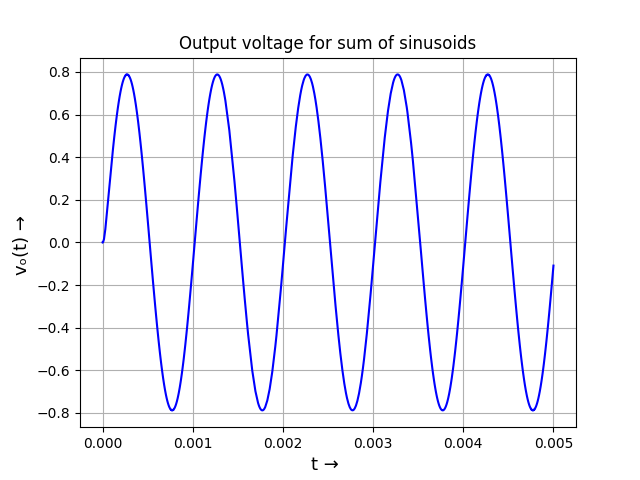
\includegraphics[scale=0.6]{Figure_2.png}
\caption{Spectrum of $f(t) = cos^3(t)$}
\label{fig:universe}
\end{figure}
\clearpage
\section{Spectrum of Frequency Modulated Wave}
Consider the signal:\newline
\begin{equation}
f(t) =  \cos(20t +5 \cos(t))    
\end{equation}

Using the same helper function as before, we get the following output:\newline
The python code for this part is:-
\begin{lstlisting}
t4 = linspace(-4*pi, 4*pi, 513); t4 = t4[:-1]
y4 = cos(20*t4 + 5*cos(t4))
Y4 = fftshift(fft(y4))/512.0
w4 = linspace(-64, 64, 513); w4 = w4[:-1]
figure(1)
# Magnitude Plot
subplot(2, 1, 1)
plot(w4, abs(Y4), lw = 2)
xlim([-30, 30])
ylabel("|Y|", size = 16)
title("Spectrum of cos(20t + 5cos(t))")
grid(True)
# Phase Plot
subplot(2, 1, 2)
ii = where(abs(Y4) > 1e-3)
plot(w4[ii], angle(Y4[ii]), 'go', lw = 2)
xlim([-30, 30])
ylabel("Phase of Y", size = 16)
xlabel("ω", size = 16)
grid(True)
show()
\end{lstlisting}
\begin{figure}[h!]
\centering
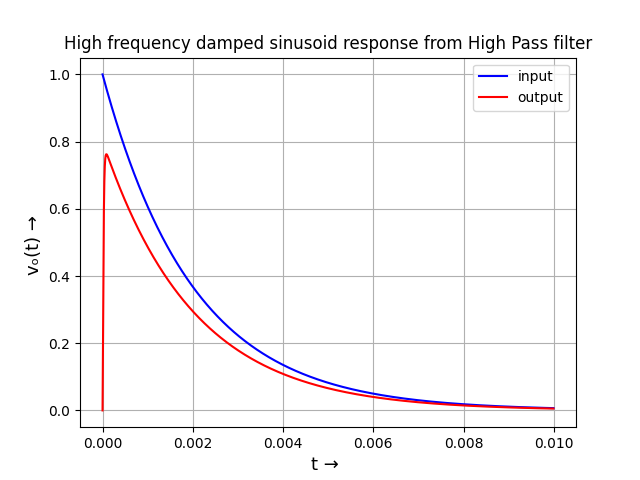
\includegraphics[scale=0.6]{Figure_4.png}
\caption{Spectrum of $f(t) = \cos(20t + 5\cos(t))$}
\label{fig:universe}
\end{figure}


The number of peaks has clearly increased. The energy in the side bands is comparable to that of the main signal.



\section{Continuous time Fourier Transform of a Gaussian}
		
The Fourier transform of a signal $x(t)$ is defined as follows:\newline
\begin{equation}
X(\omega) = \frac{1}{2 \pi} \int_{- \infty}^{\infty} x(t) e^{-j \omega t} dt    
\end{equation}


We can approximate this by the Fourier transform of the windowed version
of the signal $x(t)$, with a sufficiently large window as Gaussian curves tend to $0$ for large values of $t$ . Let the window be of size $T$. We get:
\begin{equation}
  X(\omega) \approx \frac{1}{2 \pi} \int_{- T/2}^{T/2} x(t) e^{-j \omega t} dt  
\end{equation}
On writing the integral as a Riemann sum with a small time step $\Delta t = \frac{T}{N}$, We get:
\begin{equation}
    X(\omega) \approx \frac{\Delta t}{2 \pi} \sum_{n = -\frac{N}{2}}^{\frac{N}{2}-1} x(n \Delta t) e^{-j \omega n \Delta t}
\end{equation}

Now, we sample our spectrum with a sampling period in the frequency
domain of \(\Delta \omega = \frac{2 \pi}{T}\), which makes our
continuous time signal periodic with period equal to the window size
\(T\). Our transform then becomes:
\begin{equation}
X(k \Delta \omega) \approx \frac{\Delta t}{2 \pi} \sum_{n = -\frac{N}{2}}^{\frac{N}{2}-1}x(n \Delta t) e^{-j \frac{2 \pi}{N} k n} 
\end{equation}
This form is similar to a DFT(for a finite window size). Therefore:
\begin{equation}
X(k \Delta \omega) \approx \frac{\Delta t}{2 \pi} DFT \{x(n \Delta t)\}    
\end{equation}

We made a few approximations by using a finite window size and by using the Riemann approximation

We can improve these approximations by making the window size $T$ larger, and by decreasing the time domain sampling period or increasing the number of samples $N$. We find the appropriate values for these iterative keeping the sampling frequency constant.

The expression for the Gaussian is :
\begin{equation}
    x(t) = e^{\frac{-t^2}{2}}    
\end{equation}
The CTFT is given by:
\begin{equation}
X(j \omega) = \frac{1}{\sqrt{2 \pi}}e^{\frac{-\omega^2}{2}}    
\end{equation}
\begin{lstlisting}
def gaussFn(x):
    return exp(-0.5*x**2)

def ExpectedGauss(w):
    return 1/sqrt(2*pi) * exp(-w**2/2)

def estdft(tolerance = 1e-6, samples = 128, func = gaussFn, expectedfn = ExpectedGauss, wlim = 5):
    T = 8*pi
    N = samples
    Yold = 0
    error = tolerance + 1
    iter = 0
    # Iterative loop to find window size
    while error > tolerance:  
        x = linspace(-T/2, T/2, N + 1)[:-1]
        w = linspace(-N*pi/T, N*pi/T, N + 1)[:-1]
        y = gaussFn(x)
        Y = fftshift(fft(ifftshift(y)))*T/(2*pi*N)
        error = sum(abs(Y[::2] - Yold))
        Yold = Y
        iter += 1
        T *= 2
        N *= 2
        

    # Calculating error
    true_error = sum(abs(Y - expectedfn(w))) # Absolute error
    print("True error: ", true_error)
    print("Samples = " + str(N))
    print("Time period = " + str(T))

    mag = abs(Y)
    phi = angle(Y)
    phi[where(mag < tolerance)] = 0
    
    ######
    # 6.) Plotting estimated output
    figure()
    
    # Magnitude Plot
    subplot(2, 1, 1)
    plot(w, abs(Y), lw = 2)
    xlim([-wlim, wlim])
    ylabel('Magnitude', size = 16)
    title("Estimated FFT of Gaussian")
    grid(True)

    # Phase Plot
    subplot(2, 1, 2)
    plot(w, angle(Y), 'ro', lw = 2)
    ii = where(abs(Y) > 1e-3)
    plot(w[ii], angle(Y[ii]), 'go', lw = 2)
    xlim([-wlim, wlim])
    ylabel("Phase", size = 16)
    xlabel("ω", size = 16)
    grid(True)
    show()

    #######
    # 7.) Plotting expected output    
    Y_out = expectedfn(w)
    
    mag = abs(Y_out)
    phi = angle(Y_out)
    phi[where(mag < tolerance)] = 0
    
    figure()
    
    # Magnitude Plot
    subplot(2, 1, 1)
    plot(w, abs(Y), lw = 2)
    xlim([-wlim, wlim])
    ylabel('Magnitude', size = 16)
    title("True FFT of Gaussian")
    grid(True)

    # Phase Plot
    subplot(2, 1, 2)
    plot(w, angle(Y), 'ro', lw = 2)
    ii = where(abs(Y) > 1e-3)
    plot(w[ii], angle(Y[ii]), 'go', lw = 2)
    xlim([-wlim, wlim])
    ylabel("Phase", size = 16)
    xlabel("ω",size = 16)
    grid(True)
    show()

    return


estdft()

\end{lstlisting}

\begin{figure}[h!]
\centering
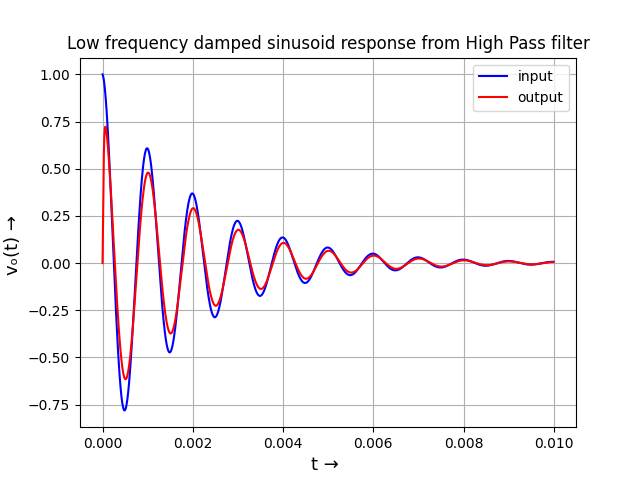
\includegraphics[scale=0.6]{Figure_5.png}
\caption{estimated CTFT of Gaussian}
\label{fig:universe}
\end{figure}

\begin{figure}[h!]
\centering
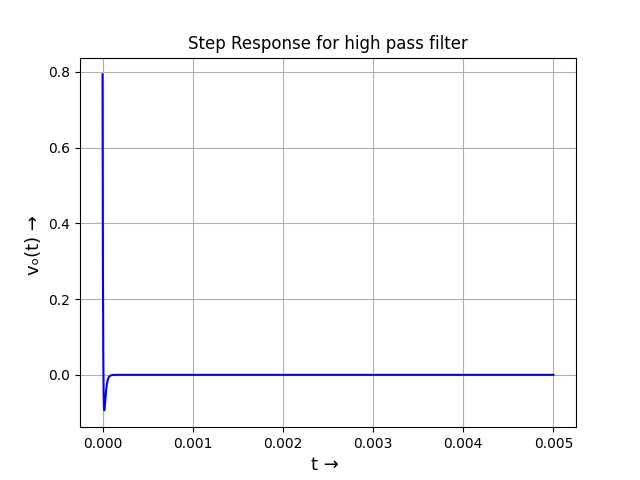
\includegraphics[scale=0.6]{Figure_6.png}
\caption{Expected CTFT of Gaussian}
\label{fig:universe}
\end{figure}
The summation of the absolute values of the error, Final number of samples and final window size are given as:\newline
True error: 1.472553842671434e-14\newline
Samples = 512\newline 
Time period = 100.53096491487338\newline

From the above pairs of plots, it is clear that with a sufficiently large window size and sampling rate, the DFT approximates the CTFT of the gaussian.This is because the magnitude of the gaussian quickly approaches 0 for large values of time.This means that there is lesser frequency domain aliasing due to windowing. Windowing in time is equivalent to convolution with a sinc in frequency domain.  A large enough window means that the sinc is tall and thin. This tall and thin sinc is approximately equivalent to a delta function for a sufficiently large window.  This means that convolution with this sinc does not change the spectrum much. Sampling after windowing is done so that the DFT can be calculated using the Fast Fourier Transform.  With sufficiently large sampling rates, this approximates the CTFT of the original time domain signal. This process is done on the gaussian and the results are in agreement with what is expected.
\clearpage

\section{Conclusion}
 The Discrete Fourier Transforms of sinusoids, amplitude modulate signals,  frequency  modulated  signals  were  analysed.   In  the  case  of  pure sinusoids,  the  DFT  contained  impulses  at  the  sinusoid  frequencies.   The amplitude modulated wave had a frequency spectrum with impulses at the carrier and the side band frequencies. The frequency moduated wave, having an infinite number of side band frequencies, gave rise a DFT with non zero values for a broader range of frequencies.  The DFT of a gaussian is also a gaussian and the spectrum was found to sharpen for higher sampling rates,while broaden for greater time ranges.



\end{document}